\chapter{Sharp Regression Discontinuity Designs}
\label{chap:rd}

\begin{description}
  \item[Motivation.] What can we learn when treatment is a deterministic
  function of a running variable?
  \item[Identification.] Why only the treatment effect at the cutoff is
  identified without additional assumptions.
  \item[Estimation.] How local linear regression estimates the two limits.
  \item[Application.] Incumbency effects in U.S. House elections.
\end{description}

\section{A deterministic treatment rule}

In earlier chapters, unconfoundedness was paired with overlap.  For a scalar
covariate $W_i$, those assumptions allowed us to compare treated and untreated
units at the same value $W_i=w$.  A sharp regression discontinuity (RD) design
is deliberately different.  Treatment obeys a deterministic rule,
\begin{equation}
  D_i=\1\{W_i\geq c\},
  \label{eq:rd-assignment}
\end{equation}
where $c$ is a known cutoff.  Conditional on $W_i$, treatment is degenerate;
there is no treated--untreated overlap except in a limiting sense at the
cutoff.  Thus the usual unconfoundedness formula
\[
  \E[Y_i\mid D_i=1,W_i=w]-\E[Y_i\mid D_i=0,W_i=w]
\]
is not well-defined: below $c$ the first conditional mean is unavailable, and
above $c$ the second is unavailable.

Write the observed outcome as
\[
  Y_i=D_iY_i(1)+(1-D_i)Y_i(0).
\]
The conditional average treatment effect is
\begin{equation}
  \tau(w)=\E[Y_i(1)-Y_i(0)\mid W_i=w].
  \label{eq:rd-cate}
\end{equation}
Away from the cutoff, one of its two components is missing:
\[
  \tau(w)=
  \begin{cases}
    \E[Y_i\mid W_i=w]-\E[Y_i(0)\mid W_i=w], & w\geq c,\\
    \E[Y_i(1)\mid W_i=w]-\E[Y_i\mid W_i=w], & w<c.
  \end{cases}
\]
Without extrapolation, therefore, we cannot identify the entire function
$\tau(\cdot)$ or the population ATE.

\section{Identification at the cutoff}
\label{sec:rd-identification}

The cutoff is special because observations can approach it from either side.
Assume that
\[
  m_d(w)=\E[Y_i(d)\mid W_i=w],\qquad d\in\{0,1\},
\]
is continuous at $c$.  Equation~\eqref{eq:rd-assignment} and consistency imply
\begin{align*}
  \lim_{w\downarrow c}\E[Y_i\mid W_i=w]&=m_1(c),\\
  \lim_{w\uparrow c}\E[Y_i\mid W_i=w]&=m_0(c).
\end{align*}
Here $w\downarrow c$ approaches from above, whereas $w\uparrow c$ approaches
from below.  Subtracting the two limits identifies
\begin{equation}
  \tau_{RD}
  \equiv \E[Y_i(1)-Y_i(0)\mid W_i=c]
  =\lim_{w\downarrow c}\E[Y_i\mid W_i=w]
   -\lim_{w\uparrow c}\E[Y_i\mid W_i=w].
  \label{eq:sharp-rd-identification}
\end{equation}

\begin{important}
RD identification comes from the deterministic assignment rule and continuity
of the untreated and treated conditional means at the cutoff.  It does not
come from the usual unconfoundedness-plus-overlap argument.
\end{important}

The continuity requirement says that, absent the change in treatment status,
the expected outcome would not jump exactly at $c$.  This is plausible when
units just above and just below the threshold are otherwise comparable.  It is
not automatic.  Other programs changing at the same cutoff, precise
manipulation of $W_i$, or a discontinuous change in the composition of units
can invalidate the design.

The estimand is local.  An RD study of a program with an income threshold
$c=\$1{,}000$, for example, estimates the effect for families at that
threshold.  It does not by itself identify the effect for families earning
$\$500$.  Whether $\tau_{RD}$ is substantively interesting is therefore a
design question, not a statistical one.

\section{Local linear estimation}
\label{sec:rd-local-linear}

Equation~\eqref{eq:sharp-rd-identification} asks for two boundary values of a
conditional mean.  Near the cutoff, approximate that mean by a different line
on each side:
\begin{align}
  Y_i&=\beta_0^+ +\beta_1^+(W_i-c)+\varepsilon_i^+,
       &&W_i\geq c,\label{eq:rd-right-line}\\
  Y_i&=\beta_0^- +\beta_1^-(W_i-c)+\varepsilon_i^-,
       &&W_i<c.\label{eq:rd-left-line}
\end{align}
Then $\beta_0^+-\beta_0^-$ approximates the discontinuity.  Equivalently, fit
one interacted regression,
\begin{equation}
  Y_i=\gamma_0+\gamma_1D_i+\gamma_2(W_i-c)
      +\gamma_3D_i(W_i-c)+\varepsilon_i,
  \label{eq:rd-local-regression}
\end{equation}
using only observations near $c$.  The mapping is
\[
  \gamma_0=\beta_0^-,\quad
  \gamma_2=\beta_1^-,\quad
  \gamma_0+\gamma_1=\beta_0^+,\quad
  \gamma_2+\gamma_3=\beta_1^+,
\]
so $\gamma_1$ is the estimated jump.

Let
\[
  X_i=\bigl(1,D_i,W_i-c,D_i(W_i-c)\bigr)',
  \qquad
  K_{hi}=K\!\left(\frac{W_i-c}{h}\right).
\]
A kernel $K$ gives greater weight to observations closer to the cutoff, and
$h>0$ is the bandwidth.  Weighted least squares solves
\begin{equation}
  \frac{1}{n}\sum_{i=1}^n K_{hi}X_i(Y_i-X_i'\widehat\gamma)=0,
  \label{eq:rd-moment}
\end{equation}
and hence
\begin{equation}
  \widehat\gamma=
  \left(\frac{1}{n}\sum_i K_{hi}X_iX_i'\right)^{-1}
  \left(\frac{1}{n}\sum_i K_{hi}X_iY_i\right).
  \label{eq:rd-wls}
\end{equation}
The RD point estimate is the second element, $\widehat\gamma_1$.

As $n$ grows, the bandwidth must shrink so the linear approximation becomes
local, but not so quickly that too few observations remain.  This creates the
usual bias--variance tradeoff:
\begin{itemize}
  \item a small $h$ reduces approximation bias but increases variance;
  \item a large $h$ uses more data but risks fitting observations for which a
        straight line is a poor approximation.
\end{itemize}
At an MSE-optimal bandwidth, the leading smoothing bias need not be negligible
for inference.  Modern practice therefore uses robust bias correction and
reports sensitivity to bandwidth and polynomial-order choices.  The older IK
bandwidth of Imbens and Kalyanaraman is useful historically, but it is not the
only or necessarily preferred modern choice.

\subsection{Covariates}

Additional pre-treatment covariates are not required for the identification
argument in Section~\ref{sec:rd-identification}.  They may improve precision
and can help diagnose whether units look comparable near the cutoff.  They
should be included in a way that preserves the local RD specification; adding
post-treatment covariates can instead change or destroy the causal estimand.

\subsection{Why not a high-order global polynomial?}

It is possible to fit separate polynomials over the entire range of $W_i$.
Such fits were common in early applications, including the descriptive Lee
figure below.  High-order global polynomials can be unstable near a boundary
and can give distant observations excessive influence.  Local linear or local
quadratic methods are normally safer for primary estimation.

\section{Application: electoral incumbency}
\label{sec:rd-lee}

Lee (2008) studies whether winning a U.S. House election raises the Democratic
candidate's vote share in the next election.  Define
\begin{itemize}
  \item the running variable as the Democratic vote-share margin in election
        $t$, recentered so zero means a tie; and
  \item the outcome as the Democratic vote share in election $t+1$.
\end{itemize}
Winning election $t$ is endogenous in the full sample: stronger candidates and
districts both win more often and perform better later.  Very close elections,
however, compare districts on opposite sides of an institutional threshold.
The discontinuity at zero in Figure~\ref{fig:rd-lee} is interpreted as the
incumbency effect under the continuity assumptions above.

\begin{figure}[tbp]
  \centering
  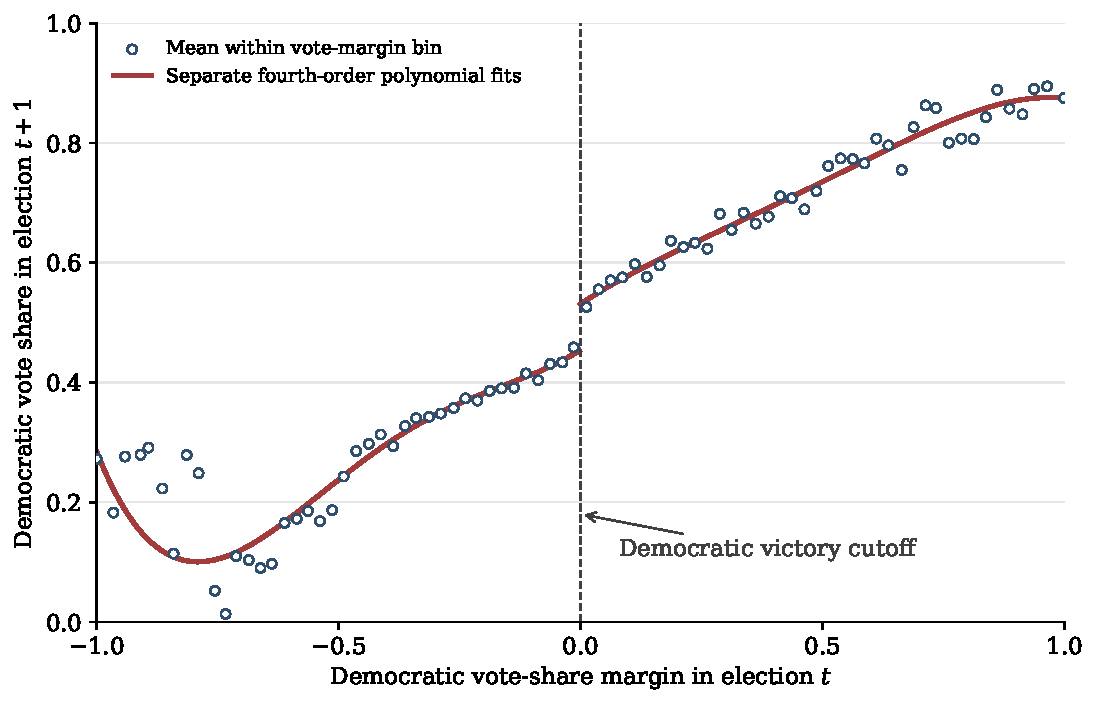
\includegraphics[width=0.88\textwidth]{../assets/Ch8RD_Lee_recreated.pdf}
  \caption{A Lee-style electoral RD illustration.  Circles are equal-width-bin
  means from the course data; curves are separate fourth-order polynomial fits
  used for visualization.  Primary estimation should use a local method.}
  \label{fig:rd-lee}
\end{figure}

Other well-known applications study mayoral wages and performance, colonial
institutions and development, financial-aid offers and college enrollment, and
angel funding and startup growth.  In every case, the central task is to defend
the institutional cutoff and the continuity of potential outcomes there.

\section{R implementation}
\label{sec:rd-r}

The following small simulation uses the \texttt{rdd} package.  Its default
\texttt{RDestimate()} call uses a triangular kernel and an automatically chosen
bandwidth.  The companion Quarto Live page runs the same code in the browser.

\begin{rcode}
library(rdd)

set.seed(5280)
x <- runif(1000, -1, 1)
y <- 3 + 2 * x + 10 * (x >= 0) + rnorm(1000)

fit_auto <- RDestimate(y ~ x)
fit_grid <- RDestimate(y ~ x,
                       bw = c(0.10, 0.20, 0.30),
                       kernel = "gaussian")
summary(fit_auto)
summary(fit_grid)
plot(fit_auto)
\end{rcode}

The Lee-style data can be loaded as follows.  The file path in the live page is
relative to the chapter file.

\begin{rcode}
library(rdd)
house <- read.csv("house.csv")
lee_local <- RDestimate(y ~ x, data = house)
summary(lee_local)
plot(lee_local)
\end{rcode}

\section*{Summary}

\begin{itemize}
  \item Sharp RD assigns treatment deterministically at a known cutoff, so
        ordinary overlap fails.
  \item Continuity identifies one local effect: the jump in the conditional
        mean of the outcome at the cutoff.
  \item Local linear regression estimates separate boundary values and avoids
        relying on a high-order global polynomial.
  \item Bandwidth choice, bias correction, manipulation, concurrent policies,
        and the local interpretation are substantive parts of the design.
\end{itemize}
